\documentclass[12pt, a4paper, oneside]{ctexart}
\usepackage{amsmath, amsthm, amssymb, bm, color, graphicx, geometry, mathrsfs,extarrows, braket, booktabs, array, mathtools}
\usepackage[colorlinks,linkcolor=red,anchorcolor=blue,citecolor=blue,urlcolor=blue,menucolor=black]{hyperref}
\setmainfont{Times New Roman}  % 设置英文字体
\setsansfont{Calibri}
\setmonofont{Consolas}

\linespread{1.4}
%\geometry{left=2.54cm,right=2.54cm,top=3.18cm,bottom=3.18cm}
\geometry{left=1.84cm,right=1.84cm,top=2.18cm,bottom=2.18cm}
\newenvironment{problem}{\par\noindent\textbf{题目. }}{\bigskip\par}
\newenvironment{solution}{\par\noindent\textbf{解答. }}{\bigskip\par}
\newenvironment{note}{\par\noindent\textbf{注记. }}{\bigskip\par}

%%%% 图片相对路径 %%%%
\graphicspath{{figure/}} % 当前目录下的figure文件夹, {../figure/}则是父目录的figure文件夹

\everymath{\displaystyle} % 默认全部行间公式
\DeclareMathOperator*\uplim{\overline{lim}} % 定义上极限 \uplim_{}
\DeclareMathOperator*\lowlim{\underline{lim}} % 定义下极限 \lowlim_{}
\let\leq=\leqslant % 将全部leq变为leqslant
\let\geq=\geqslant % geq同理

% 一些宏定义
\def\bd{\boldsymbol}        % 加粗(向量) boldsymbol
\def\disp{\displaystyle}    % 使用行间公式 displaystyle(默认)
\def\tsty{\textstyle}       % 使用行内公式 textstyle
\def\sign{\text{sign}}      % sign function
\def\wtd{\widetilde}        % 宽波浪线 widetilde
\def\R{\mathbb{R}}          % Real number
\def\N{\mathbb{N}}          % Natural number
\def\Z{\mathbb{Z}}          % Integer number
\def\C{\mathbb{C}}          % Complex number
\def\d{\mathrm{d}}          % differential operator
\def\e{\mathrm{e}}          % Euler's number
\def\i{\mathrm{i}}          % imaginary number
\def\re{\mathrm{Re}}        % Real part
\def\im{\mathrm{Im}}        % Imaginary part
\def\res{\mathrm{Res}}      % Residue
\def\L{\mathcal{L}}         % Loss function
\def\wdh{\widehat}          % 宽帽子 widehat
\def\ol{\overline}          % 上横线 overline
\def\ul{\underline}         % 下横线 underline
\def\add{\vspace{1ex}}      % 增加行间距
\def\del{\vspace{-3.5ex}}   % 减少行间距

%%% 概率论 %%%
\def\pra{\xrightarrow{\ \ p\ }}     % 右箭头上加p
\def\Lra{\xrightarrow{\ \ L\ }}     % 右箭头上加L
\def\dra{\xrightarrow{\ \ d\ }}     % 右箭头上加d
\def\P{\textbf{P}}      % Probability
\def\E{\textbf{E}}      % Exception
\def\var{\textbf{Var}}  % variance
\def\cov{\textbf{Cov}}  % covariance

% 基本信息
\newcommand{\RQ}{\today} % 日期
\newcommand{\km}{概率论} % 科目
\newcommand{\bj}{强基数学002} % 班级
\newcommand{\xm}{吴天阳} % 姓名
\newcommand{\xh}{2204210460} % 学号

\begin{document}

%\pagestyle{empty}
\pagestyle{plain}
\vspace*{-15ex}
\centerline{\begin{tabular}{*5{c}}
    \parbox[t]{0.25\linewidth}{\begin{center}\textbf{日期}\\ \large \textcolor{blue}{\RQ}\end{center}} 
    & \parbox[t]{0.2\linewidth}{\begin{center}\textbf{科目}\\ \large \textcolor{blue}{\km}\end{center}}
    & \parbox[t]{0.2\linewidth}{\begin{center}\textbf{班级}\\ \large \textcolor{blue}{\bj}\end{center}}
    & \parbox[t]{0.1\linewidth}{\begin{center}\textbf{姓名}\\ \large \textcolor{blue}{\xm}\end{center}}
    & \parbox[t]{0.15\linewidth}{\begin{center}\textbf{学号}\\ \large \textcolor{blue}{\xh}\end{center}} \\ \hline
\end{tabular}}
\vspace*{4ex}

% 正文部分
\paragraph*{习题6.1\quad 1.}试证明 (2) $X_n\pra X,\ X_{n}\pra Y\Rightarrow \P\{X=Y\} = 1$;

(10) $X_n\pra X,\ Y$是随机变量$\Rightarrow X_nY\pra XY$;

(11) $X_n\pra X,\ Y_n\pra Y\Rightarrow X_nY_n\pra XY$.
\begin{proof}
    (1) 对任意的$\varepsilon,\delta > 0$, 有
    \begin{align*}
        &\ \P(|X_n-X|\geq \frac{\varepsilon}{2})\leq \frac{\delta}{2},\ \P(|X_n-Y|\geq \frac{\varepsilon}{2})\leq \frac{\delta}{2}\\
        \Rightarrow&\ \P(|X-Y|\geq \varepsilon)\leq \P(|X_n-X|\geq \frac{\varepsilon}{2})+ \P(|X_n-Y|\geq \frac{\varepsilon}{2})\leq \delta\\
        \Rightarrow&\ \P(|X-Y|< \varepsilon) > 1-\delta.
    \end{align*}
    由$\varepsilon, \delta$的任意性可知, $\P(X=Y) = 1$.

    (10) 对任意的$\varepsilon,\delta > 0$, 由于$\P(Y < \infty) = 1$, 于是存在$M>0$使得$\P(|Y|\geq M) \leq \frac{\delta}{2}$, 且有
    \begin{equation*}
        \P(|X_n-X|\geq \frac{\varepsilon}{M})\leq \frac{\delta}{2},
    \end{equation*}
    所以
    \begin{align*}
        \P(|X_nY-XY|\geq \varepsilon)  =&\ \P(|Y||X_n-X|\geq \varepsilon)\\
        =&\ \P\left(|Y||X_n-X|\geq \varepsilon\biggl||Y|\geq M\right) + \P\left(|Y||X_n-X|\geq \varepsilon\biggl||Y| < M\right)\\
        =&\ \frac{\delta}{2} + \P\left(|Y||X_n-X|\geq \varepsilon\biggl||Y| < M\right)\\
        \leq&\ \frac{\delta}{2} + \P\left(|X_n-X|\geq \frac{\varepsilon}{M}\right)\leq \delta.
    \end{align*}
    所以$X_nY\pra XY$.

    (11) 对任意的$\varepsilon, \delta > 0$, 由(10)有
    \begin{align*}
        &\ \P(|X_n(Y_n-Y)|\geq\frac{\varepsilon}{2}) < \frac{\delta}{2},\ \P(|Y(X_n-X)|\geq \frac{\varepsilon}{2}) < \frac{\delta}{2}\\
        \Rightarrow&\ \P(|X_nY_n-X_nY|+|X_nY-XY|\geq \varepsilon) < \delta\\
        \Rightarrow&\ \P(|X_nY_n-XY|\geq \varepsilon) < \delta.
    \end{align*}
    所以$X_nY_n\pra XY$.
\end{proof}
\paragraph*{3.}设随机变量$X_n$服从Cauchy分布, 其密度函数为
\begin{equation*}
    p_n(x) = \frac{n}{\pi(1+n^2x^2)},\quad n\geq 1,
\end{equation*}
证明: $X_n\pra 0$.
\begin{proof}
    对于任意的$\varepsilon > 0$, 有
    \begin{align*}
        \P(|X_n|\geq \varepsilon) =&\  2\int_{\varepsilon}^\infty\frac{n}{\pi(1+n^2x^2)}\,\d x = \frac{2}{\pi}\arctan (nx)\biggl|_{\varepsilon}^\infty\\
        =&\  \frac{2}{\pi}\left(\frac{\pi}{2}-\arctan(n\varepsilon)\right)\to 0\quad(n\to\infty).
    \end{align*}
    所以$\lim_{n\to\infty}\P(|X_n|\geq \varepsilon) = 0\Rightarrow X_n\pra 0$.
\end{proof}
\paragraph*{7.}设$\{X_n:n\geq 1\}$是独立的随机变量序列, (由于概率之和不为0, 修改了一下题目)
\begin{align*}
    &\ \P(X_n=1)=\P(X_n=-1)=\frac{1}{2}\left(1-\frac{1}{2^n}\right),\\
    &\ \P(X_n=n)=\P(X_n=-n)=\frac{1}{2^{k+1}},\quad k=n+1,n+2,\cdots.
\end{align*}
试问: $\{X_n:n\geq 1\}$是否服从弱大数定律?
\begin{solution}
    服从. 由于$P(X_n=a) = P(X_n=-a)$, 所以$\E X_n = 0$, 
    \begin{equation*}
        \E X_n^2 = \left(1+\frac{1}{2^n}\right)+\sum_{k=n+1}^\infty\frac{k^2}{2^k}\leq 1+\sum_{k=1}^\infty\frac{k^2}{2^k}\leq 1+\frac{x(1+x)}{(1-x)^3}\biggl|_{x=\frac{1}{2}} = 7 < \infty.
    \end{equation*}
    由Chebyshev弱大数定律得证.
\end{solution}
\paragraph*{10.}设在Bernoulli试验序列中, 事件$A$出现的概率为$p$, 令
\begin{equation*}
    X_n=\begin{cases}
        1,\quad\text{在第}n\text{次及第}n+1\text{次试验中}A\text{都出现},\\
        0,\quad\text{其他},
    \end{cases}
\end{equation*}
则$\{X_n,n\geq 1\}$服从弱大数定律.
\begin{proof}
    由于$X_n$与$X_{n+1}$有相关性, 无法直接使用Chebyshev弱大数定理, 每个$X_n$均为参数为$p^2$的Bernoulli变量, 所以$\E X_n = p^2,\ \E X_n^2 = p^2,\ \var X_n = p^2(1-p^2)$, 且
    \begin{equation*}
    \cov X_iX_j = \begin{cases}
        p^3 - p^4,&\quad |i-j| = 1,\\
        0,&\quad |i-j| \geq 2.
    \end{cases}
    \end{equation*}
    
    设$S_n = \sum_{k=1}^nX_k$, 于是
    \begin{equation*}
        \var S_n = \sum_{k=1}^n\var X_n + 2\sum_{i=1}^n\cov(X_i,X_{i+1}) = np^2(1-p^2) + 2(n-1)p^3(1-p).
    \end{equation*}
    故$\lim_{n\to\infty}\frac{\var S_n}{n^2} = 0$, 由Markov弱大数定理得证.
\end{proof}

\paragraph*{习题6.2\quad 4.}若$\bd{X}_n$为$n$维正态随机向量, $\bd{X}_n\pra \bd{X}$, 试证$\bd{X}$为正态向量.
\begin{proof}
    由于$X_n\pra X$, 则$X_n\dra X$, 于是$\lim_{n\to\infty}F_n(x) = F(x)$, 其中$F_n(x),\ F(x)$分别为$X_n,\ X$的分布函数, 由于$X_n$为$n$为正态随机变量, 所以$X$为正态向量.
\end{proof}
\paragraph*{6.}设$\{X_n\}$依分布收敛到$X$, 设$\{Y_n\}$依分布收敛到常数$a$, 证明$X_n+Y_n$依分布收敛到$X+a$.
\begin{solution}
    设$F(x) = \P(X+a\leq x) = \P(X\leq x - a)$, 由于$Y_n\pra a$, 则$\forall \varepsilon > 0$, $\forall x\in C(F)$, $\exists\varepsilon_1\in(0,\varepsilon)$, 使得$x\pm \varepsilon_1\in C(F)$, 令$T_n=X_n+Y_n$, 于是
    \begin{align*}
        \P(T_n\leq x) =&\ \P(T_n\leq x,|Y_n-a|\leq \varepsilon_1)+\P(T_n\leq x,|Y_n-a|>\varepsilon_1)\\
        \leq&\ \P(X_n\leq x-a+\varepsilon_1)+\P(|Y_n-a| > \varepsilon_1),
    \end{align*}
    所以$\uplim_{n\to\infty}\P(T_n\leq x) \leq F(x+\varepsilon_1)$, 又由于
    \begin{align*}
        \P(X_n\leq x-a-\varepsilon_1) =&\ \P(X_n\leq x-a-\varepsilon_1,|Y_n-a|\leq\varepsilon_1)+\P(X_n\leq x-a-\varepsilon_1,|Y_n-a| > \varepsilon_1)\\
        \leq&\ \P(T_n\leq x)+\P(|Y_n-a| > \varepsilon_1),
    \end{align*}
    所以$\lowlim_{n\to\infty}\P(T_n\leq x)\geq F(x-\varepsilon_1)$. 综上
    \begin{equation*}
        F(x-\varepsilon_1)\leq \lowlim_{n\to\infty}\P(T_n\leq x)\leq \uplim_{n\to\infty}\P(T_n\leq x)\leq F(x+\varepsilon_1),
    \end{equation*}
    当$\varepsilon\to0$时, $\lim_{n\to\infty}\P(T_n\leq x) = F(x),\ (x\in C(F))$, 故$X_n+Y_n=T_n\dra x+a$.
\end{solution}
\paragraph*{7.}设$\{X_k\}$为独立随机变量序列, 它们都服从$-1$与$1$两点上的等可能分布. 试证$Y_n=\sum_{k=1}^n\frac{X_k}{2^k}$依分布收敛到$U(-1,1)$随机变量.
\begin{proof}
    设$f_n(t)$为$Y_n$的特征函数, 则
    \begin{equation*}
        f_{Y_n}(t) = \E\exp\left\{\i t\sum_{k=1}^n\frac{X_k}{2^k}\right\} = \prod_{k=1}^n\E\exp\left\{\i t\frac{X_k}{2^k}\right\} = \prod_{k=1}^n f_{X_k}\left(\frac{t}{2^k}\right).
    \end{equation*}
    对任意$k\in[1, n]$时, 有$f_{X_k}(t) = \E\exp\{\i tX_k\} = \int_{-\infty}^{\infty}\e^{\i tx}\,\d F(X_k) = \frac{e^{\i t}+\e^{-\i t}}{2} = \cos t$. 于是
    \begin{equation*}
        f_{Y_n}(t) = \prod_{k=1}^nf_{X_k}\left(\frac{t}{2^k}\right) = \prod_{k=1}^n\cos \frac{t}{2^k}.
    \end{equation*}
    由于
    \begin{align*}
        2^n\sin\left(\frac{t}{2^n}\right)f_{Y_n}(t) = 2^n\prod_{k=1}^n\cos\frac{t}{2^k}\sin\frac{t}{2^n} =&\ 2^n\cos\frac{t}{2}\cos\frac{t}{2^2}\cdots\cos\frac{t}{2^n}\sin\frac{t}{2^n}\\
        =&\ 2^{n-1}\cos\frac{t}{2}\cos\frac{t}{2^2}\cdots\cos\frac{t}{2^{n-1}}\sin\frac{t}{2^{n-1}}\\
        =&\ \cdots=\sin t,
    \end{align*}
    则$f_{Y_n}(t) = \frac{\sin t}{2^n\sin\frac{t}{2^n}}$, 所以
    \begin{equation*}
        \lim_{n\to\infty}f_{Y_n}(t) = \lim_{n\to\infty}\frac{\sin t}{2^n\sin\frac{t}{2^n}} = \frac{\sin t}{t}.
    \end{equation*}

    再设$Y\sim U(-1,1)$, 则
    \begin{equation*}
        f_{Y}(t) = \int_{-\infty}^\infty \e^{\i tx}\,\d F_Y(x) = \int_{-1}^1\frac{\e^{\i tx}}{2}\,\d x = \frac{\e^{\i t}-\e^{-\i t}}{2\i t} = \frac{\sin t}{t}.
    \end{equation*}

    由于$\lim_{t\to 0}\frac{\sin t}{t} = 1$, 所以$f(t)$在$0$处连续且$\lim_{n\to\infty}f_{Y_n}(t) = f_Y(t)$, 由连续性定理知
    \begin{equation*}
        \sum_{k=1}^n\frac{X_k}{2^k}=Y_n\dra Y=U(-1,1).
    \end{equation*}
\end{proof}
\paragraph*{8.}设$X_n\pra X$, 而$g$是$\R^1$上的连续函数, 试证$g(X_n)\pra g(X)$.
\begin{proof}
    由$g$的连续性可知, $\forall \varepsilon >0 $, 存在$\delta > 0$, 使得当$|x_n-x| <\delta$时, 有$|g(x_n)-g(x)| < \varepsilon$, 于是
    \begin{align*}
        &\ \{|X_n-X|< \delta\}\subset \{|g(X_n) - g(X)|< \varepsilon\}\\
        \Rightarrow&\ \{|g(X_n) - g(X)|\geq \varepsilon\}\subset \{|X_n-X|\geq \delta\}\\
        \Rightarrow&\ \P(|g(X_n) - g(X)|\geq \varepsilon)\leq \P(|X_n-X|\geq \delta)\to 0\quad(n\to \infty)\\
        \Rightarrow&\ g(X_n)\pra g(X).
    \end{align*}
\end{proof}
\paragraph*{习题6.3\quad 1.}设$\{X_n:n\geq 1\}$是独立同分布的随机变量序列, $\E X_1 = a$, 则对直线上任一有界连续函数$f(x)$,
\begin{equation*}
    \lim_{n\to\infty}\E f\left(\frac{X_1+\cdots+X_n}{n}\right) = f(a).
\end{equation*}
\begin{proof}
        由Khinchin弱大数律可知
        \begin{align*}
            &\ \frac{X_1+\cdots+X_n}{n}\pra a\\
            \xRightarrow[\text{习题6.2\ 8.}]{f\text{连续}}&\ f\left(\frac{X_1+\cdots+X_n}{n}\right)\pra f(a)\\
            \xRightarrow[\text{Lebesgue控制收敛定理}]{f\text{有界}}&\ \E f\left(\frac{X_1+\cdots+X_n}{n}\right)\to f(a)\quad(n\to\infty)
        \end{align*}
\end{proof}

% 下面给一些功能的写法
\iffalse
% 图片模板
\centerline{
    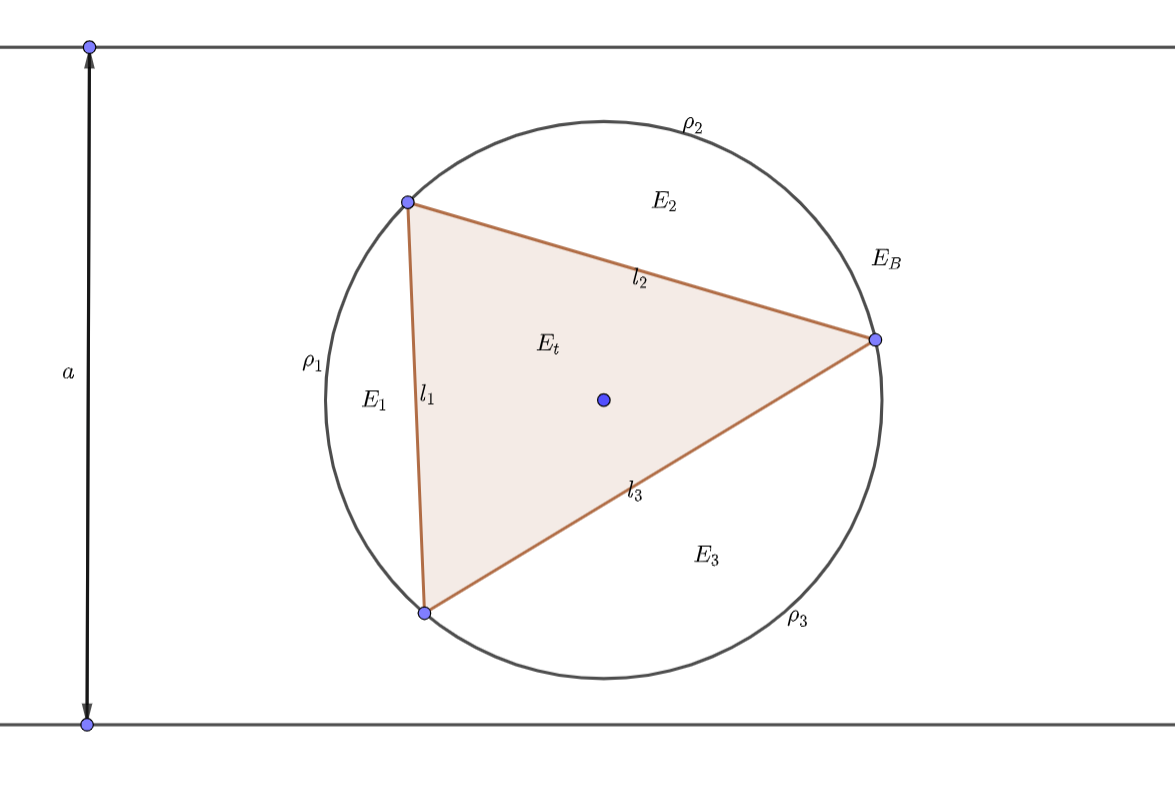
\includegraphics[width=0.8\textwidth]{figure.png}
}
% 表格模板
\renewcommand\arraystretch{0.8} % 设置表格高度为原来的0.8倍
\begin{table}[!htbp] % table标准
    \centering % 表格居中
    \begin{tabular}{p{1cm}<{\centering}p{1cm}<{\centering}p{3cm}<{\centering}p{5cm}<{\centering}} % 设置表格宽度
    %\begin{tabular}{cccc}
        \toprule
        $x_i$ & $f[x_1]$ & $f[x_i,x_{i+1}]$ & $f[x_i,x_{i+1},x_{i+2}]$ \\
        \midrule
        $x_0$ & $f(x_0)$ &                  &                          \\
        $x_0$ & $f(x_0)$ & $f'(x_0)$        &                          \\
        $x_0$ & $f(x_1)$ & $\frac{f(x_1)-f(x_0)}{x_1-x_0}$ & $\frac{f(x_1)-f(x_0)}{(x_1-x_0)^2}-\frac{f'(x_0)}{x_1-x_0}$\\
        \bottomrule
    \end{tabular}
\end{table}

\def\Log{\text{Log}} % 一个简单的宏定义
$\Log$ % 调用方法
\fi

\end{document}